%! Author = t.kramer
%! Date = 10/06/2023


% \pagebreak
\section{comfortSIM}

To test the feasibility of the created framework, we developed a prototype implementation called \textit{comfortSIM}, or comfort \textbf{S}imulation \textbf{I}nterface \textbf{M}odule. \textit{comfortSIM} is an open-source Python module that serves as a bridge between data-driven thermal comfort prediction and simulation tools such as Ladybug Tools. Based on spatially resolved indoor climate data, it integrates the last four components of the developed framework, thus making it easier to incorporate them into comfort modelling workflows. 

Rather than being a simulation tool in itself, \textit{comfortSIM} is an array-based code structure that facilitates the connection between thermal simulation, data science and \gls{ml}. The module is based on Numpy \citep{vanderWaltNumpy2011}, a Python library to numerically compute large data sets and perform mathematical operations on multidimensional arrays or matrices. 

Data from indoor thermal environments can be represented as multidimensional arrays that carry hourly data points. Using Numpy, performing operations on this grid-based data related to thermal comfort and simulated indoor climate becomes computationally highly efficient. The matrix-based approach facilitates key computational processes such as pre-processing, model training, and post-processing. Furthermore, relying on a straightforward but flexible matrix structure, \textit{comfortSIM} enables the integration of various simulation software, programming languages, and open source \gls{ml} and data science libraries. 

The following sections provide a brief overview of how the proposed framework components were implemented in \textit{comfortSIM}. For more details, please refer to the GitHub repository listed at the end of this paper.


%%%%%%%%%%%%%%%%%%%%%%%%%%%%%%%%%%%%%%%%%%%%%%

\subsection{Spatial mapping algorithm}

To achieve a grid-based simulation output, we used a mapping algorithm implemented in Ladybug Tools \citep{SadeghipourRoudsariLadybug2013}. The method for spatial mapping of indoor environmental conditions was developed by \citet{Mackey2015} and uses a simplified algorithm in EnergyPlus and its native EPW weather files \citep{CrawleyEnergyPlus2001} to calculate spatially resolved indoor environmental parameters on Radiance sensor grids, all while considering the influence of short-wave and long-wave solar radiation. 


%%%%%%%%%%%%%%%%%%%%%%%%%%%%%%%%%%%%%%%%%%%%%%

\subsection{Offset classification}
\label{sec:classification}

To account for the variability in the perception of thermal comfort between individuals, we decided to use the ASHRAE Global Thermal Comfort Database II \citep{Foldvary2018} as a basis for classifying the perception of thermal comfort. Based on previous findings \citep{KramerFieldstudy2023}, we used a subset of the database containing only personalised samples with an existing subject ID.

First, for the entire dataset, we plotted \gls{set} in 0.1 K bins against the \gls{tsv} parameter and fitted a third-degree polynomial function through the data points. The resulting function in \Cref{eq:tsv-predicted} describes the overall relationship between measured \gls{set} and \gls{tsv} present in the ASHRAE subset (see \Cref{fig:offset}.a). 

\begin{equation}\label{eq:tsv-predicted}
   \text{TSV}_{\text{predicted}} = f\text{(SET)}  
\end{equation}

\begin{equation}\label{eq:mean-offset}
   \text{Subject mean offset} = \sum_{i=1}^{n} (TSV_{actual,i} - TSV_{predicted,i})
\end{equation}

Next, we moved to a personalised analysis and calculated the difference or "offset" between the predicted \gls{tsv} as estimated using the newly developed function and the actual \gls{tsv} as submitted by individual subjects in the ASHRAE database. We then used the calculated offset values to determine the mean personal offset (\Cref{eq:mean-offset}) for each subject and visualised their distribution in a histogram (see \Cref{fig:offset}.b). After inspecting the distribution, we decided to separate the data into five bins, or "offset classes". These offset classes, ranging from -2 to +2, classify subjects represented in the ASHRAE subset into different persona types based on the deviation from the overall \gls{tsv} comfort function.

For subjects assigned to a positive offset class (e.g., subjects in classes +1 and +2), the developed \gls{tsv} function underestimates their perception of thermal comfort. They tend to feel warmer and prefer cooler conditions than indicated by the majority vote. Vice versa, subjects with a negative mean offset (classes -1 and -2) tend to feel cooler and prefer warmer conditions than their fellow occupants. The thermal sensation of subjects in class 0, the neutral and predominant class, can be adequately described by the developed function. They are likely to perceive thermal conditions similarly to the majority of occupants. 


\begin{figure*}[!h]
    \centering
    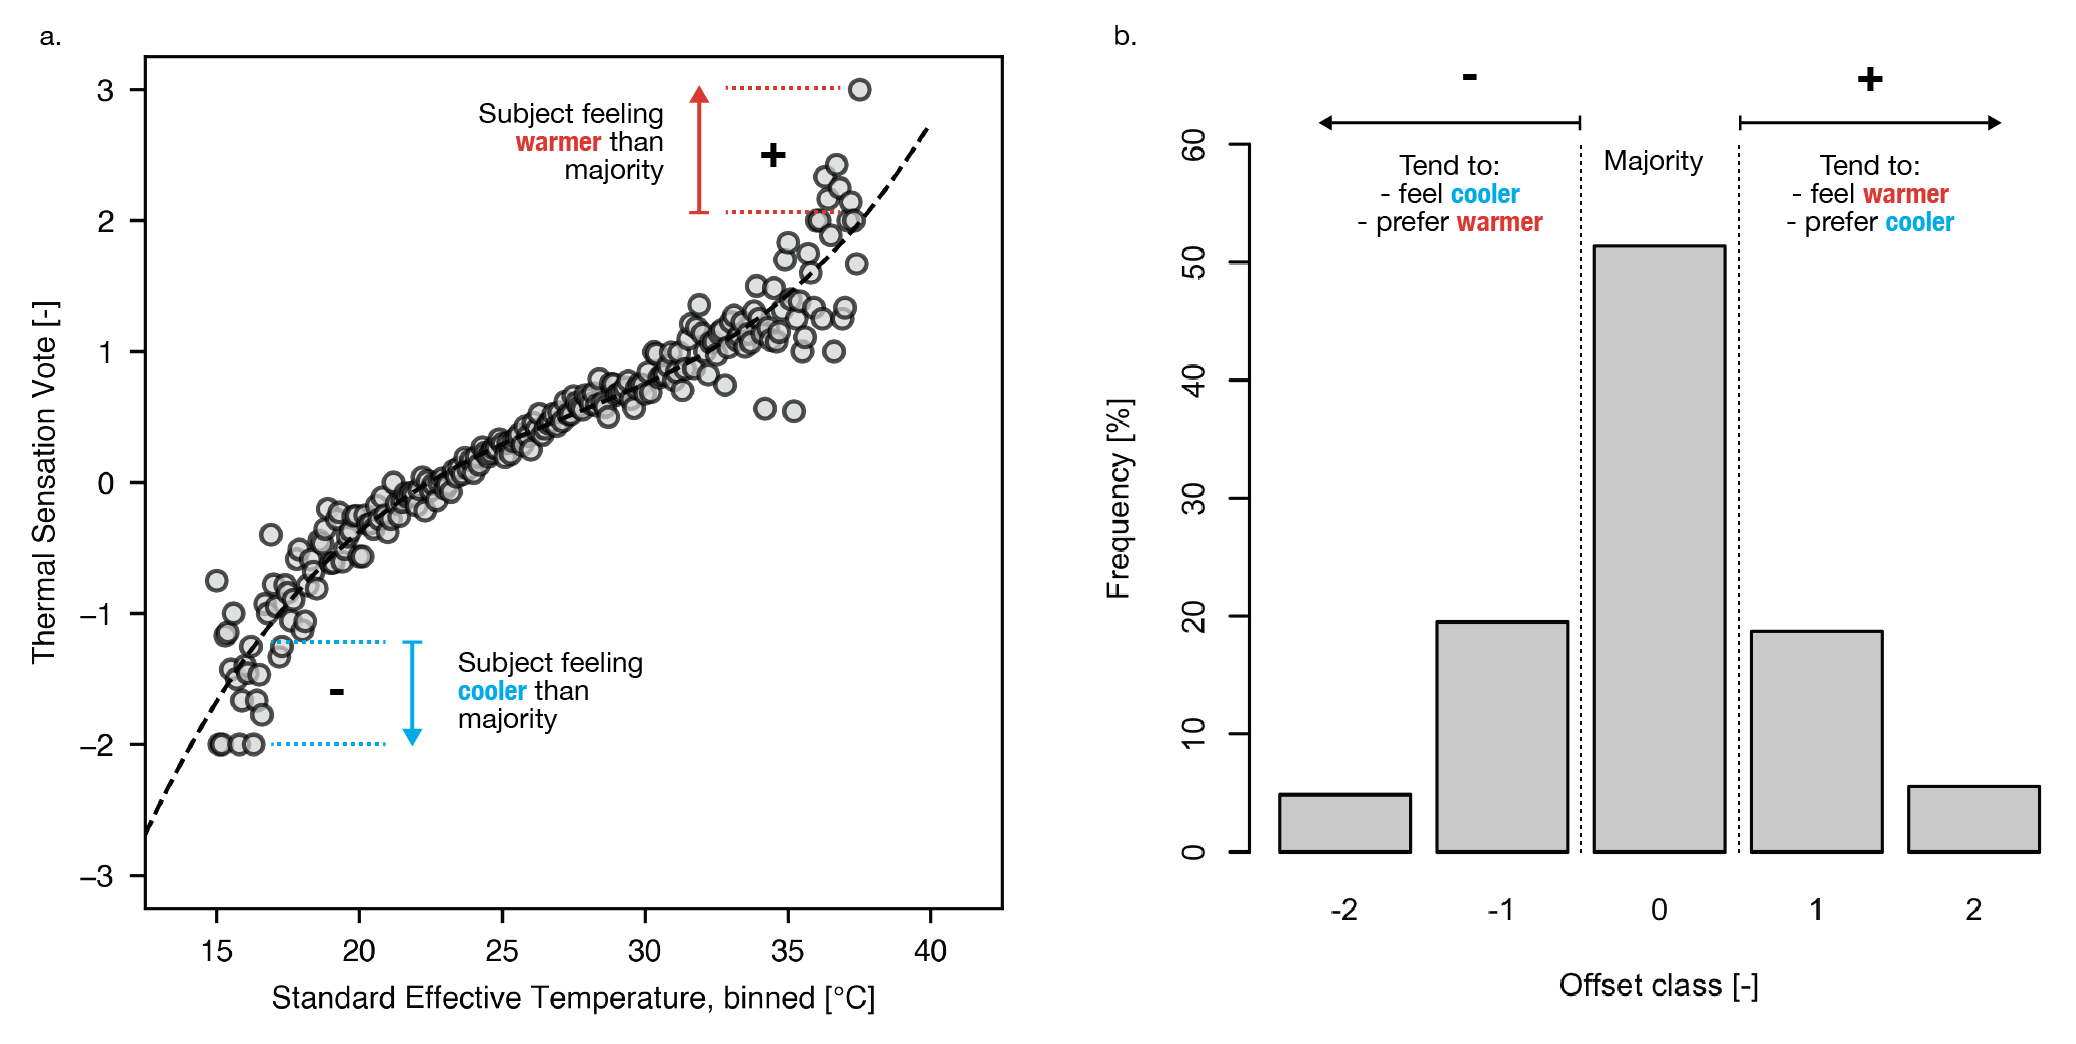
\includegraphics[width=\textwidth]{manuscript/src/figures/offset-class.png}
    \caption{Offset classification: (a) 3rd degree polynomial relationship between binned Standard Effective Temperature (SET) and Thermal Sensation Vote (TSV) with examples of negative and positive offset; (b) Normally distributed offset classes in ASHRAE subset containing only personalised samples with existing 'subject-id'; based on the mean deviation from the polynomial function in (a), each participant was classified into one out of five offset classes, ranging from -2 to +2.}
    \label{fig:offset}
\end{figure*}

In practice, the derived classification scheme can be used to evaluate thermal comfort for several types of persona with different perceptions and preferences for comfort. We decided to use the offset classes as input parameters for a data-driven thermal preference classifier. Here, predicting the expected thermal preference for different persona types allows for a more nuanced assessment of thermal comfort and demonstrates the variability thermal preference, for example, between occupants preferring warmer conditions (classes -2 and -1) and those who generally prefer cooler environments (+1 and +2)


%%%%%%%%%%%%%%%%%%%%%%%%%%%%%%%%%%%%%%%%%%%%%%

\subsection{Data-driven thermal preference model}

Next, we use the generated offset classes as a feature to train a \gls{ml}-based thermal preference prediction model. Although \gls{tsv} is still the predominant label for the prediction of thermal comfort, thermal preference is a dependent variable that is more closely related to the actions of the occupants and their preferred comfort state. Therefore, selecting thermal preference as target variable links the model predictions with the inclination of the occupants to use \gls{pcs}.

We designed the model to solve a classification problem. For each grid point, and based on the simulated environmental conditions, the thermal preference classifier predicts the probability of three target classes, ‘cooler’ (-1), ‘warmer’ (1), or ‘no change’ [0], for each offset class. We deliberately focused on the detection of discomfort and identified classes that indicate a preferred change in environmental conditions (-1, 1) as positive classes. To optimise \gls{tpr} for positive classes (-1, 1), we selected \textit{Recall} as the primary prediction accuracy metric \citep{James2013}. Additionally, we recorded and plotted the Area Under the Receiver Operating Characteristic Curve (AUC). The results of a performance test comparing a selection of \gls{ml} algorithms are reported in \Cref{sec:results-ml}.


%%%%%%%%%%%%%%%%%%%%%%%%%%%%%%%%%%%%%%%%%%%%%%

\subsection{PCS integration via OOP}

We propose the use of \gls{oop}-based \gls{pcs} objects (as visualised in \Cref{fig:pcs-oop}) to integrate their effect into the simulation workflow. After defining typical personal comfort devices such as desktop fans or foot warmers as Python objects with attributes and methods describing their distinct properties and influence on personal thermal comfort, we used these objects to updated the simulated indoor climate data via post-processing.

In the \textit{comfortSIM} method, the thermal preference classifier predicts the expected thermal preference for the simulated environmental conditions simulated at each grid point and for each offset class. Next, combining the results of these predictions allows identifying locations and offset classes of potential spatial discomfort. The \gls{pcs} objects' methods and attributes can be used to update the indoor environmental conditions stored in each matrix element via post-processing.

After overwriting the indoor environmental parameters based on the heating or cooling effects (also known as "corrective power") of \gls{pcs}, e.g., as reported in \citep{ZhangHui2015}, the updated indoor climate dataset can then be used to re-predict thermal preference using the updated conditions. This creates a loop that allows evaluating the effect of several \gls{pcs} devices on indoor environmental conditions, and consequently the expected spatial thermal preference of an occupant sitting in that position.


\begin{figure}[H]
    \centering
    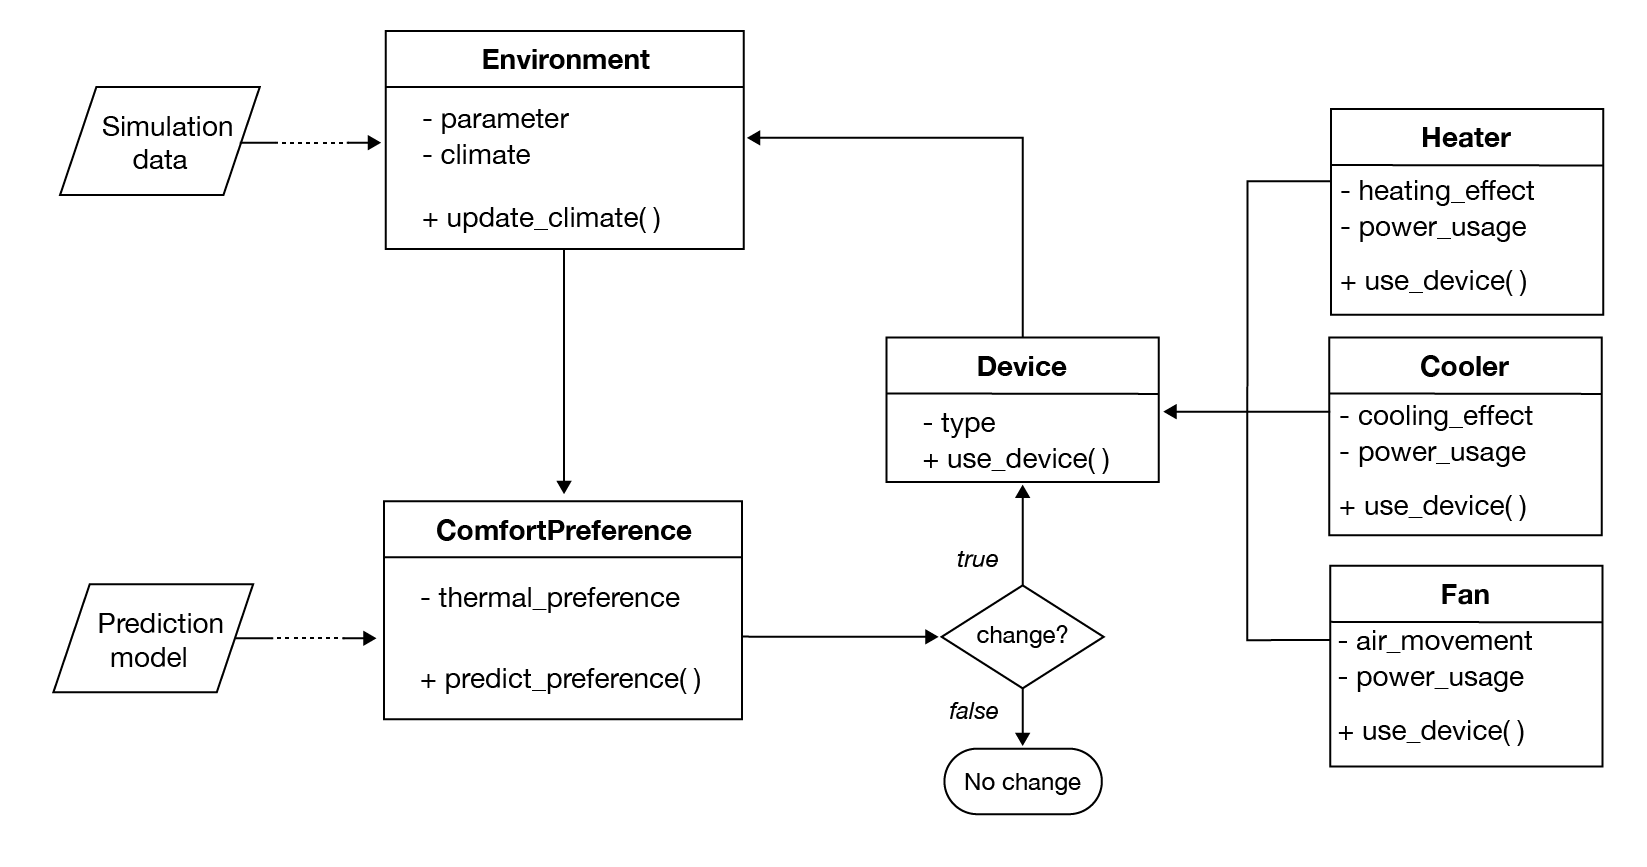
\includegraphics[width=\linewidth]{manuscript/src/figures/pcs-oop-flowchart.png}
    \caption{Conceptual Unified Modelling Language (UML) diagram of \gls{pcs} definitions with classes, attributes and methods based on the approach of object-oriented programming (OOP): Based on an Environment class, ComfortPreferences are predicted and used as a basis for a Boolean decision if the Environment.climate has to be adjusted by a Device class object, e.g. a Heater, Cooler or Fan.}
    \label{fig:pcs-oop}
\end{figure}



%%%%%%%%%%%%%%%%%%%%%%%%%%%%%%%%%%%%%%%%%%%%%%

\subsection{spatial Thermal Autonomy}

\citet{Levitt2013} introduced the term "Thermal Autonomy” or TA, which denotes: "the percent of occupied time over a year where a thermal zone meets or exceeds a given set of thermal comfort acceptability criteria through passive means only". We propose an amendment to the initial idea and suggest using \gls{sta} as a novel metric for the evaluation of thermal comfort in the building planning stages.

Following a similar index in the field of daylight, the spatial Daylight Autonomy or sDA introduced by \citet{Heschong2012}, we define \gls{sta} as the "percentage of floor area during occupied time over a year where a thermal zone meets or exceeds a given set of thermal comfort acceptability criteria through passive means and \gls{pcs} only”. For example, the percentage of floor area during occupied time over a year where a thermal zone is within 19 and 27\degree {C} only by using passive strategies and \gls{pcs} such as desk fans or heated chairs. Here, we support the inclusion of \gls{pcs} that facilitate individual thermal comfort and adaptation.

The benefits of using \gls{sta} as a long-term index for thermal comfort design include:


\begin{itemize}

    \item \gls{sta} retains the simplicity of other metrics and provides additional informative value by combining spatial and temporal dimension;
    
    \item \gls{sta} as a metric facilitates the evaluation and comparison of the performance of comfort-related building design without mechanical systems and leads to a refocus on the building and occupants;
    
    \item \gls{sta} can help identify problematic areas in the thermal zone investigated and is a fundamental prerequisite for planning the deployment of \gls{pcs};

    % \item if generated following a data-driven method, the increased capabilities in data science and \gls{ai} will facilitate the adoption of a learning process that takes advantage of the data collected in existing buildings to improve the thermal autonomy of future buildings. 
    
\end{itemize}

\subsubsection*{Practical implications}

As pointed out in the introduction, our aim was to propose a flexible framework that can be implemented software-independently. The entire framework, including the proposed implementation in \textit{comfortSIM}, is entirely based on openly available software packages and is therefore fully reproducible. Moreover, the development of \textit{comfortSIM} as a post-processing package facilitates flexible use in combination with other simulation tools that can generate a grid- or array-based output. The developed package provides a flexible interface using multidimensional arrays for analysis, prediction, and visualisation.

The way the framework is implemented is flexible. Under different circumstances, such as other training data sets or input features, different \gls{ml} algorithms may be more efficient and the prediction problem can be defined differently. This, however, does not affect the power of \gls{ml} as a promising alternative to conventional models such as \gls{pmv} or \gls{acm}.

With regard to the practical application of our work, the framework should be interpreted as such. To be a viable alternative to conventional approaches in practise, more underlying data is required for further validation and optimisation. However, architects, engineers, and designers can leverage the insights gained from our research to question their conventional workflows and to embrace the opportunities presented by data-driven applications in the built environment.